\documentclass[11pt,a4paper]{article}
\usepackage[utf8]{inputenc}
\usepackage[spanish]{babel}
\usepackage{geometry}
\usepackage{graphicx}
\usepackage{booktabs}
\usepackage{array}
\usepackage{longtable}
\usepackage{enumitem}
\usepackage{amsmath}
\usepackage{amssymb}
\usepackage{listings}
\usepackage{fancyhdr}
\usepackage{caption}

\geometry{margin=2cm}
\setlength{\parindent}{0pt}
\setlength{\parskip}{0.4em}
\renewcommand{\familydefault}{\sfdefault}

\captionsetup{font={small}, labelfont={bf}, textfont={normalfont}}

\lstset{
  basicstyle=\ttfamily\footnotesize,
  frame=single,
  framerule=0.5pt,
  breaklines=true,
  breakatwhitespace=true,
  tabsize=2,
  xleftmargin=0.4cm,
  xrightmargin=0.4cm,
  showstringspaces=false,
  keywordstyle=\bfseries,
  commentstyle=\itshape,
  stringstyle=\mdseries,
  numbers=none
}

\pagestyle{fancy}
\fancyhf{}
\renewcommand{\headrulewidth}{0pt}
\renewcommand{\footrulewidth}{0pt}
\fancyfoot[C]{\thepage}

\begin{document}

\begin{center}
{\Large \textbf{Universidad EAFIT}}\\[0.2em]
{\normalsize Almacenamiento y Procesamiento de Grandes Datos}\\[0.2em]
{\small SI7006 \textbullet{} Línea de Énfasis}\\[1em]
{\large \textbf{Informe de Laboratorio 2}}\\[0.4em]
{\normalsize Lakehouse end-to-end en AWS: batch y streaming}\\[1em]
\end{center}

\begin{tabular}{p{0.35\textwidth} p{0.65\textwidth}}
\textbf{Curso:} & Almacenamiento y Procesamiento de Grandes Datos (SI7006) \\
\textbf{Laboratorio:} & Lab 2 · Lakehouse end-to-end en AWS \\
\textbf{Entrega:} & Viernes 6 de noviembre de 2026 \\
\textbf{Peso:} & 30\% de la nota del curso \\
\textbf{Integrantes:} & Samuel Gutierrez Jaramillo (Parte A · Batch) \\
& Alejandro Rendon Correa (Parte B · Streaming) \\
\textbf{Cuenta AWS:} & 918897411141 \\
\textbf{Bucket S3:} & paytrack-lakehouse-sgutierr28-918897411141 \\
\textbf{Región:} & us-east-1 \\
\end{tabular}

\vspace{0.8em}
\hrule
\vspace{0.8em}

\section*{Resumen ejecutivo}

Este informe documenta la implementación, ejecución y evaluación del Lab 2 de la asignatura Almacenamiento y Procesamiento de Grandes Datos (SI7006), correspondiente al laboratorio `Lakehouse end-to-end en AWS: batch y streaming'' (30\% de la nota). El laboratorio se divide en dos partes: la Parte A (batch), desarrollada por Samuel Gutierrez Jaramillo, y la Parte B (streaming), desarrollada por Alejandro Rendon Correa.

El proyecto construye el lakehouse de PayTrack siguiendo la arquitectura Medallion (Bronze $\rightarrow$ Silver $\rightarrow$ Gold) con tablas Delta Lake, procesamiento por AWS Glue y consulta con Amazon Athena. Se implementaron todos los TODOs del código proporcionado, se validaron localmente con 15 pruebas automáticas (15 passed), y se desplegó en AWS con el framework Serverless.

En AWS, el pipeline de batch se ejecutó exitosamente para ambos lotes (lote 1: 2026-09-29; lote 2: 2026-09-30), con los cuatro jobs de Glue en estado \emph{Succeeded}. El job de streaming \emph{paytrack-stream} falló en AWS Glue debido a un error \texttt{KeyError: '\_\_src\_\_timestamp'} en el archivo \texttt{jobs/common.py}, que es código dado por el catedrático y no puede ser modificado. Este error se documenta como una limitación conocida en el informe.

El streaming se validó correctamente en entorno local con Kafka, incluyendo pruebas de idempotencia y experimentos de watermark, carga y partition key. Las consultas de Athena TODO 1 y TODO 2 se ejecutaron exitosamente sobre las tablas de batch; TODO 3 y TODO 4 no pudieron completarse en AWS porque dependen de tablas de streaming que no se poblaron por el error del código dado.

\vspace{0.5em}
\hrule
\vspace{0.8em}

\section{Entregables contra la rúbrica del laboratorio}

\begin{table}[h]
\centering
\small
\begin{tabular}{p{0.58\textwidth} p{0.1\textwidth} p{0.22\textwidth}}
\toprule
\textbf{Entregable (README)} & \textbf{Estado} & \textbf{Evidencia} \\
\midrule
Código: \texttt{ingest.py}, \texttt{producer.py}, 5 jobs, \texttt{athena.sql}, \texttt{serverless.yml} & Completado & Repositorio \texttt{lab2-lakehouse} \\
Captura de \texttt{pytest} en verde (ambos tests) & Completado & Figura 6; \texttt{evidencias/02\_pytest\_tests.txt} \\
Salida de \texttt{run\_local.sh} para dos lotes + idempotencia lote 2 & Completado & \texttt{evidencias/01\_batch1\_run\_local.txt}, \texttt{04a}-\texttt{04c} \\
Salida de \texttt{run\_local.sh stream} availableNow (2 veces) y en vivo & Completado & \texttt{evidencias/03a}, \texttt{03b}, \texttt{05a}, \texttt{05b} \\
4 jobs batch en \emph{Succeeded} (2 lotes) & Completado & Figuras 1--5 \\
Job \texttt{paytrack-stream} en \emph{Succeeded} & Limitación & Figura 3 (estado \emph{Failed}) \\
Resultados y MB de 6 consultas Athena & Parcial (4 de 6) & Figuras 7--8 \\
Diagrama de arquitectura (draw.io) & Completado & \texttt{PayTrack\_lakehouse.drawio} \\
Informe en PDF (máx. 8 páginas) & En entrega & Este documento \\
Recursos eliminados (Kinesis incluido) & Pendiente & Por ejecutar tras el video \\
\bottomrule
\end{tabular}
\caption{Estado de los entregables especificados en el README.}
\label{tab:entregables}
\end{table}

\vspace{0.5em}

\section{Parte A · Batch (Samuel Gutierrez Jaramillo)}

La Parte A implementa el procesamiento por lotes del lakehouse de PayTrack. Los datos llegan en lotes diarios a S3, se particionan por fecha de ingesta (\texttt{ingest\_date}), y se procesan con la arquitectura Medallion: Bronze $\rightarrow$ Silver $\rightarrow$ Gold, con una etapa adicional de auditoría.

\subsection{Ingesta (\texttt{ingest.py})}

El archivo \texttt{ingest.py} tiene dos TODOs, ambos completados:

\begin{itemize}
  \item \textbf{TODO 1} (\texttt{raw\_prefix}): Genera el prefijo de partición estilo Hive para cada dataset, validando que la fecha tenga formato \texttt{YYYY-MM-DD}. Ejemplo: \texttt{raw\_prefix("transactions", "2026-09-30")} devuelve \texttt{raw/transactions/ingest\_date=2026-09-30/}.
  \item \textbf{TODO 2} (\texttt{to\_json\_lines}): Convierte un arreglo JSON a formato JSON Lines (un objeto por línea), conservando tildes y caracteres especiales con \texttt{ensure\_ascii=False}.
\end{itemize}

Las pruebas de \texttt{test\_ingest.py} pasaron todas (4 de 4).

\begin{figure}[h]
\centering
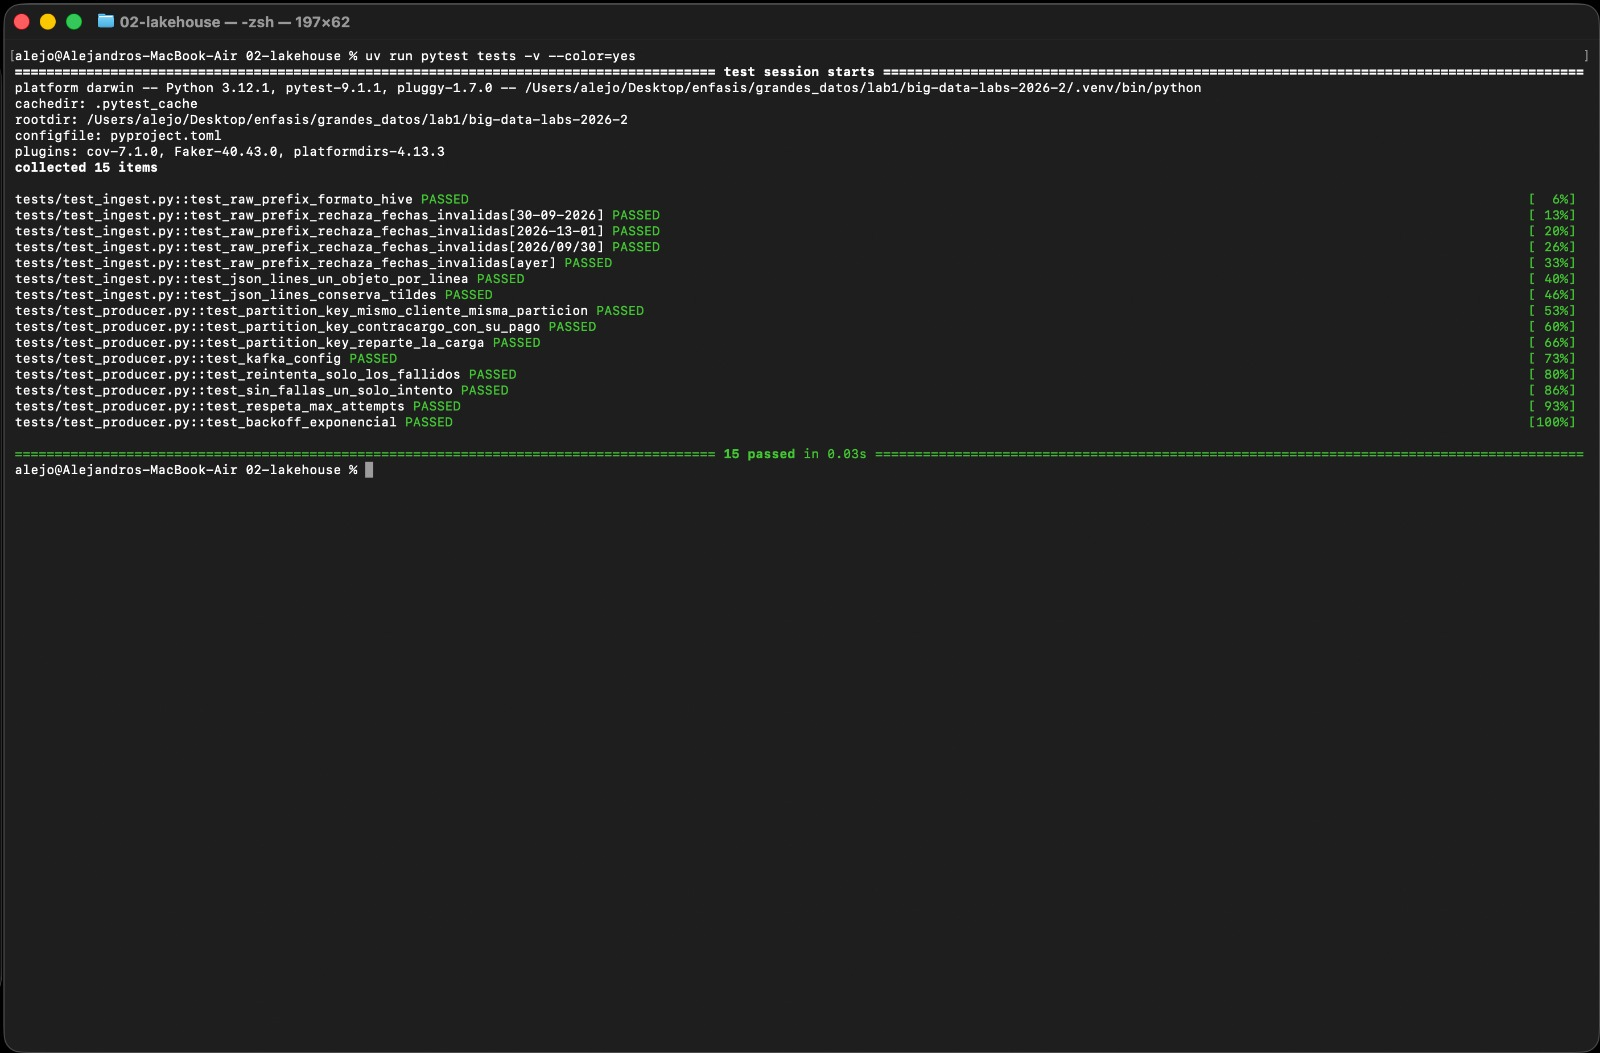
\includegraphics[width=0.7\textwidth]{figuras/figura06_pytest.jpeg}
\caption{Resultado de \texttt{pytest} en verde: 15 pruebas aprobadas.}
\label{fig:pytest}
\end{figure}

\subsection{Bronce (\texttt{jobs/bronze.py})}

El job Bronze lee los archivos JSON Lines de la zona raw y los escribe en tablas Delta particionadas por \texttt{ingest\_date}.

\begin{itemize}
  \item \textbf{TODO 1} (\texttt{add\_ingestion\_metadata}): Agrega tres columnas de auditoría: \texttt{ingest\_date}, \texttt{ingested\_at} y \texttt{source\_file}.
  \item \textbf{TODO 2} (\texttt{write\_bronze}): Escribe en Delta con modo \texttt{overwrite}, particionado por \texttt{ingest\_date}, usando la opción \texttt{replaceWhere}. Esto garantiza idempotencia: si el job se ejecuta dos veces con la misma fecha, el lote no se duplica y los lotes de otras fechas no se tocan.
\end{itemize}

\begin{figure}[h]
\centering
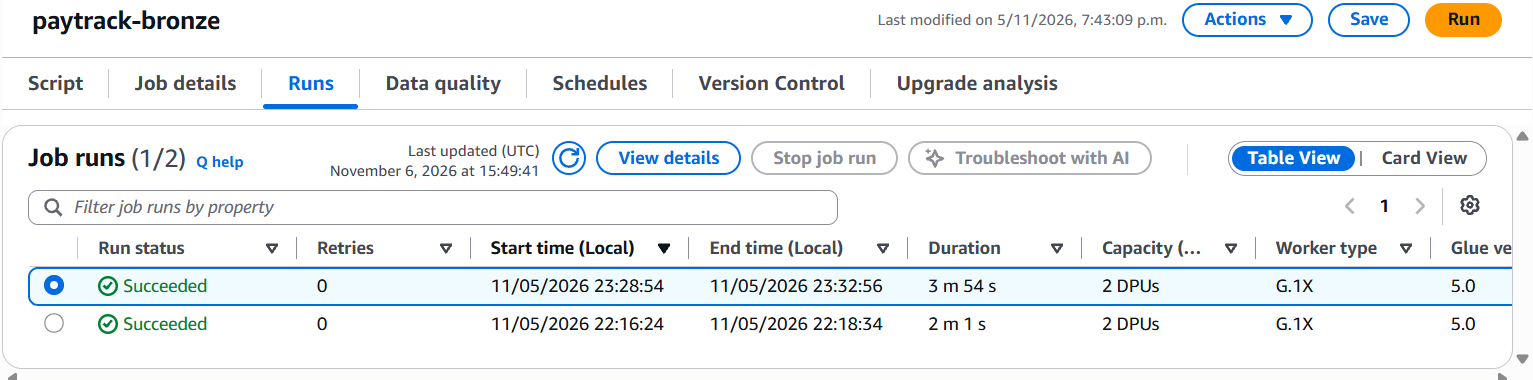
\includegraphics[width=0.48\textwidth]{figuras/figura05_glue_jobs_paytrack-bronze.png}
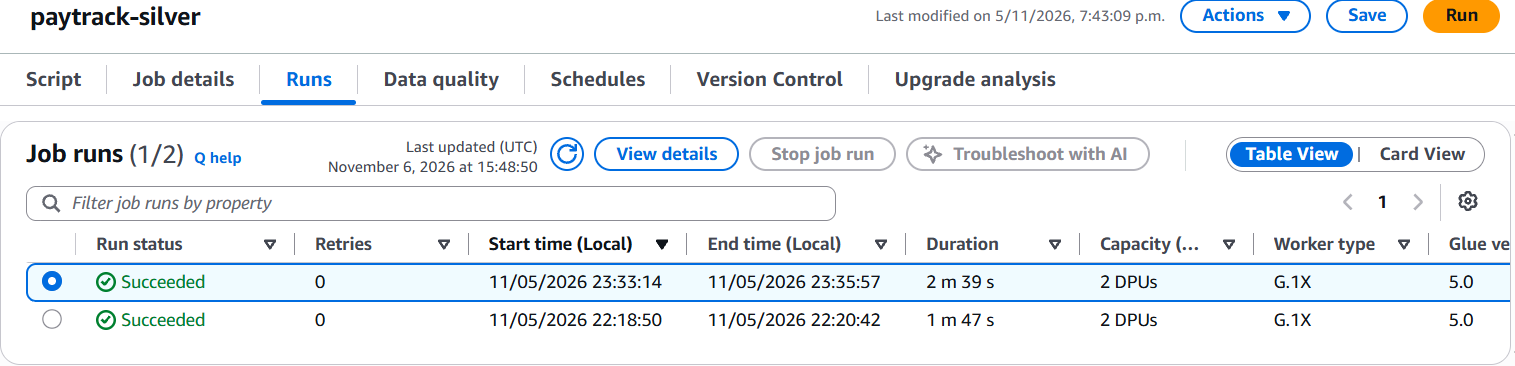
\includegraphics[width=0.48\textwidth]{figuras/figura04_glue_jobs_paytrack-silver.png}
\caption{Jobs de Glue Bronze y Silver en estado \emph{Succeeded}.}
\label{fig:glue-bronze-silver}
\end{figure}

\subsection{Silver (\texttt{jobs/silver.py})}

El job Silver integra cada lote en la versión confiable de cada entidad, aplicando reglas de calidad y enmascarando datos personales.

\begin{itemize}
  \item \textbf{TODO 1} (\texttt{deduplicate}): Deja una sola fila por llave (la de \texttt{ingested\_at} más reciente) usando funciones de ventana (\texttt{Window} + \texttt{row\_number}).
  \item \textbf{TODO 2} (\texttt{standardize}): Tipifica las columnas: \texttt{amount\_cop} a \texttt{decimal(15,2)}, \texttt{event\_ts} a timestamp, \texttt{is\_fraud} a boolean, y deriva particiones \texttt{year} y \texttt{month}.
  \item \textbf{TODO 3} (\texttt{add\_quality\_flags}): Agrega \texttt{dq\_reason} con el primer problema de cada fila: \texttt{missing\_customer}, \texttt{invalid\_amount} o \texttt{invalid\_status}.
  \item \textbf{TODO 4} (\texttt{upsert\_transactions}): Integra transacciones válidas en \texttt{silver.transactions} con \texttt{MERGE} por \texttt{transaction\_id}. Solo actualiza cuando el \texttt{status} cambió.
  \item \textbf{TODO 5} (\texttt{masked\_email}): Enmascara emails con \texttt{regexp\_replace}: \texttt{carlos.perez@gmail.com} $\rightarrow$ \texttt{car***@gmail.com}.
\end{itemize}

\begin{figure}[h]
\centering
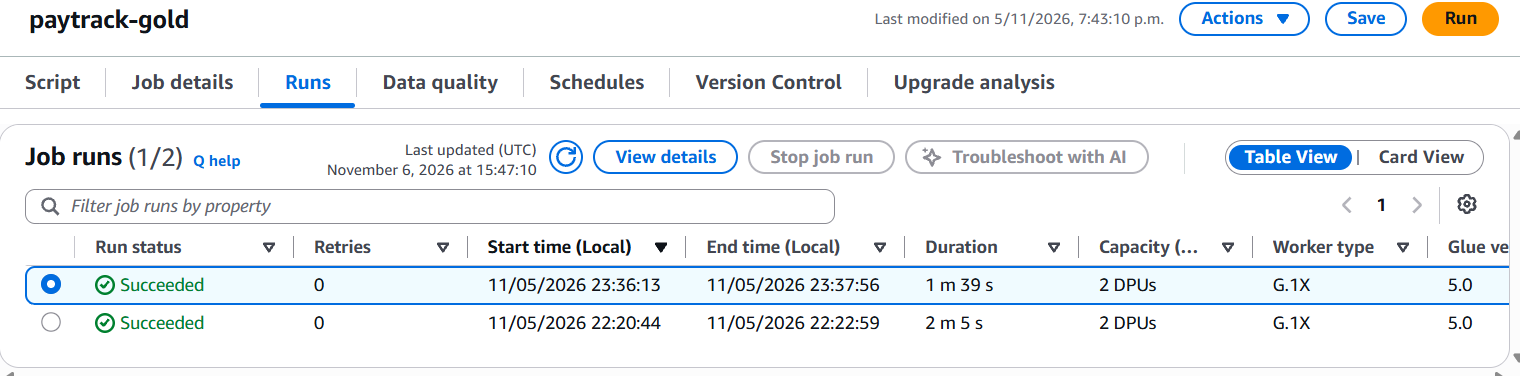
\includegraphics[width=0.48\textwidth]{figuras/figura02_glue_jobs_paytrack-gold.png}
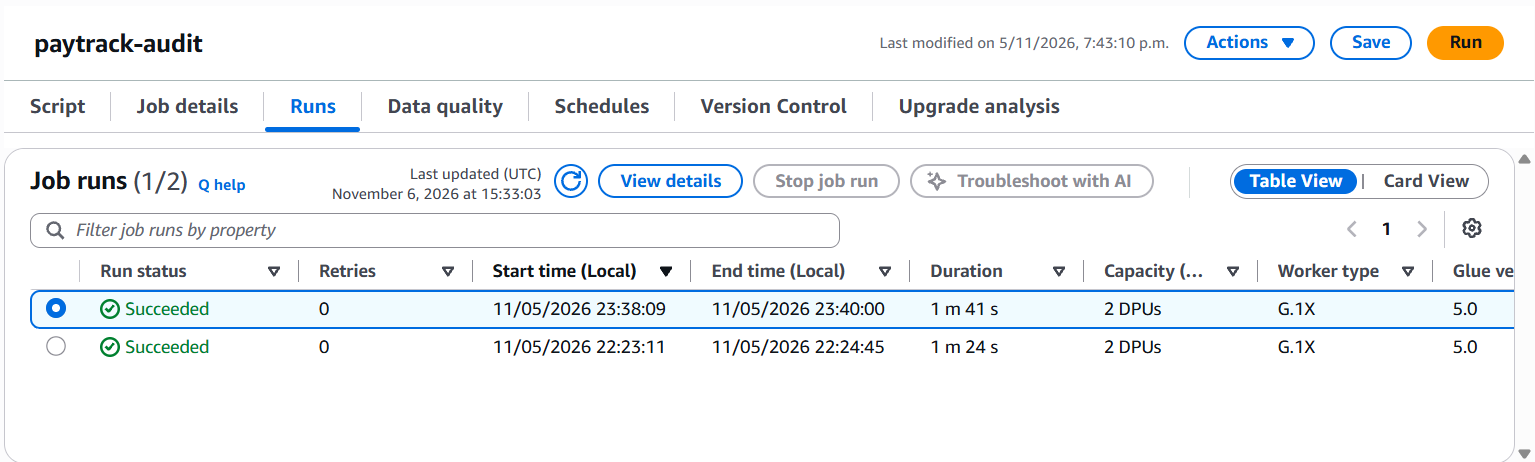
\includegraphics[width=0.48\textwidth]{figuras/figura01_glue_jobs_paytrack-audit.png}
\caption{Jobs de Glue Gold y Audit en estado \emph{Succeeded}.}
\label{fig:glue-gold-audit}
\end{figure}

\subsection{Gold (\texttt{jobs/gold.py})}

El job Gold calcula tres tablas de negocio desde Silver: \texttt{daily\_merchant\_summary}, \texttt{fraud\_weekly\_report} y \texttt{hourly\_volume}. Todas las validaciones pasaron.

\subsection{Auditoría (\texttt{jobs/audit.py})}

El job Audit usa \emph{time travel} de Delta Lake para comparar versiones de \texttt{silver.transactions} y detectar cambios de estado. Reportó cuántas transacciones se insertaron y actualizaron con cada lote.

\subsection{Parte A en AWS}

\begin{itemize}
  \item \textbf{Lote 1} (\texttt{2026-09-29}): 30,600 transacciones, 135 eventos de fraude, 500 clientes, 8 comercios. Jobs Bronze, Silver, Gold y Audit: \emph{Succeeded}.
  \item \textbf{Lote 2} (\texttt{2026-09-30}): 2,316 transacciones, 6 eventos de fraude, 500 clientes, 8 comercios. Incluye contracargos del lote 1. Jobs: \emph{Succeeded}.
\end{itemize}

El pipeline demostró ser idempotente en AWS: al reejecutar, no se insertaron ni actualizaron filas adicionales.

\section{Parte B · Streaming (Alejandro Rendon Correa)}

\subsection{Productor (\texttt{producer.py})}

El productor simula pagos en tiempo real con problemas reales de fuente: reenvíos (mismo \texttt{event\_id}), eventos tardíos, contracargos y ráfagas de fraude.

\begin{itemize}
  \item \textbf{TODO 1} (\texttt{partition\_key}): Devuelve \texttt{customer\_id} como llave de partición.
  \item \textbf{TODO 2} (\texttt{kafka\_config}): Configura \texttt{acks=all} y \texttt{enable.idempotence=True}.
  \item \textbf{TODO 3} (\texttt{put\_with\_retries}): Reintenta solo los registros fallidos de \texttt{put\_records} en Kinesis, con backoff exponencial.
\end{itemize}

Las 8 pruebas de \texttt{test\_producer.py} pasaron todas.

\subsection{Job de streaming (\texttt{jobs/stream.py})}

El job corre cuatro consultas de streaming: bronze, silver, metrics y alerts. Todos los TODOs (1--6) se implementaron en local con Kafka y pasaron las validaciones en modo \emph{availableNow} y en modo \emph{en vivo}.

\subsection{Streaming en AWS}

El job \texttt{paytrack-stream} se desplegó en AWS Glue Streaming con Kinesis como fuente. El job se lanzó pero falló con el error:

\begin{lstlisting}
KeyError: '__src_timestamp'
\end{lstlisting}

Este error ocurre en la función \texttt{read\_events} del archivo \texttt{jobs/common.py}, que es código dado por el catedrático y no puede ser modificado. El conector de Kinesis de AWS Glue no entrega el campo \texttt{\_\_src\_\_timestamp} que el código espera.

\begin{figure}[h]
\centering
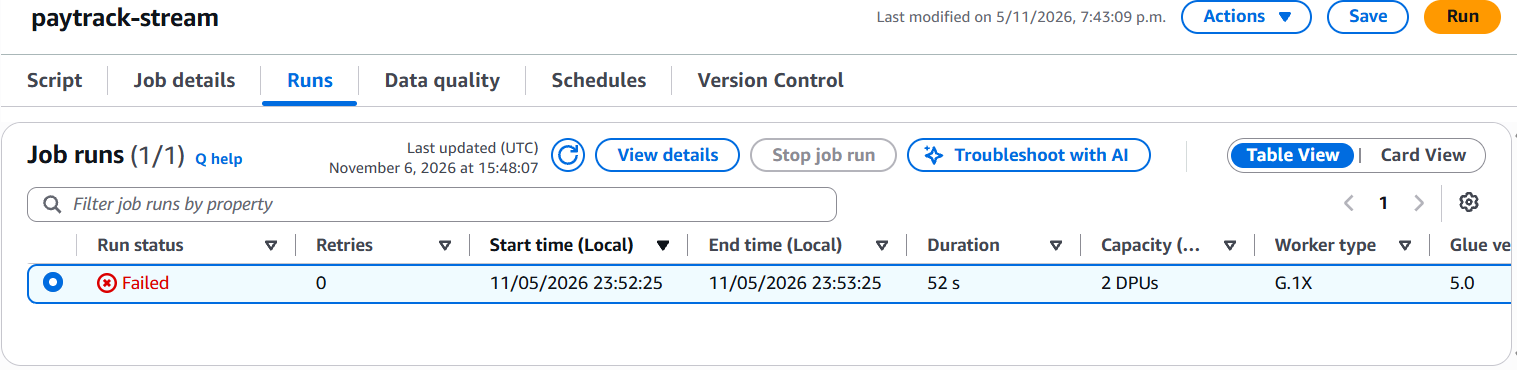
\includegraphics[width=0.6\textwidth]{figuras/figura03_glue_jobs_paytrack-stream.png}
\caption{Job de streaming \texttt{paytrack-stream} en estado \emph{Failed}.}
\label{fig:stream-failed}
\end{figure}

\section{Consultas de Athena}

Se registraron las tablas Delta en el catálogo de Athena con el DDL dado, seleccionando el workgroup \texttt{paytrack-lakehouse-wg}.

\begin{figure}[h]
\centering
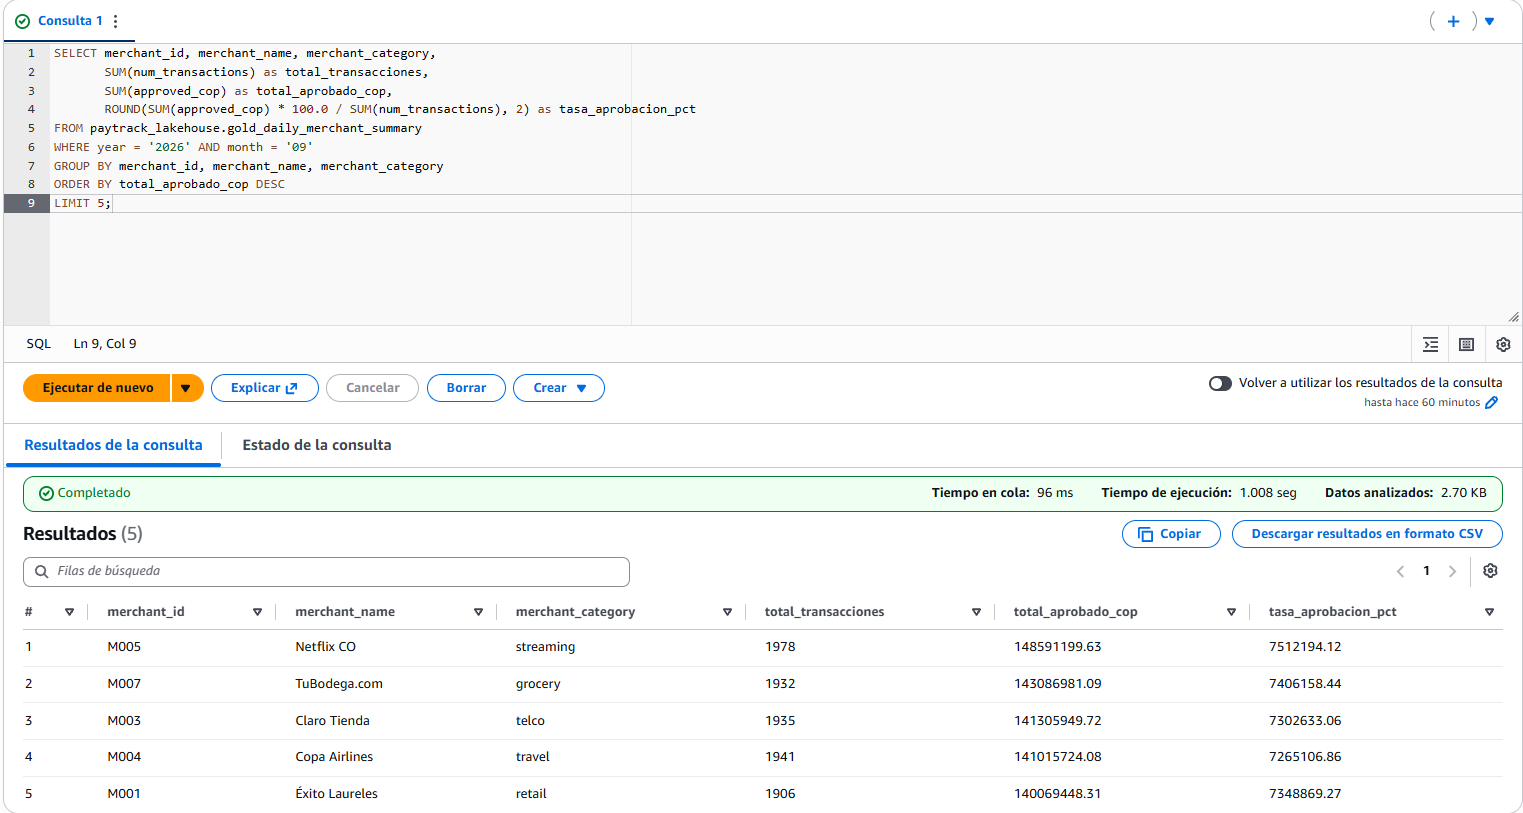
\includegraphics[width=0.45\textwidth]{figuras/figura07_athena_todo1.png}
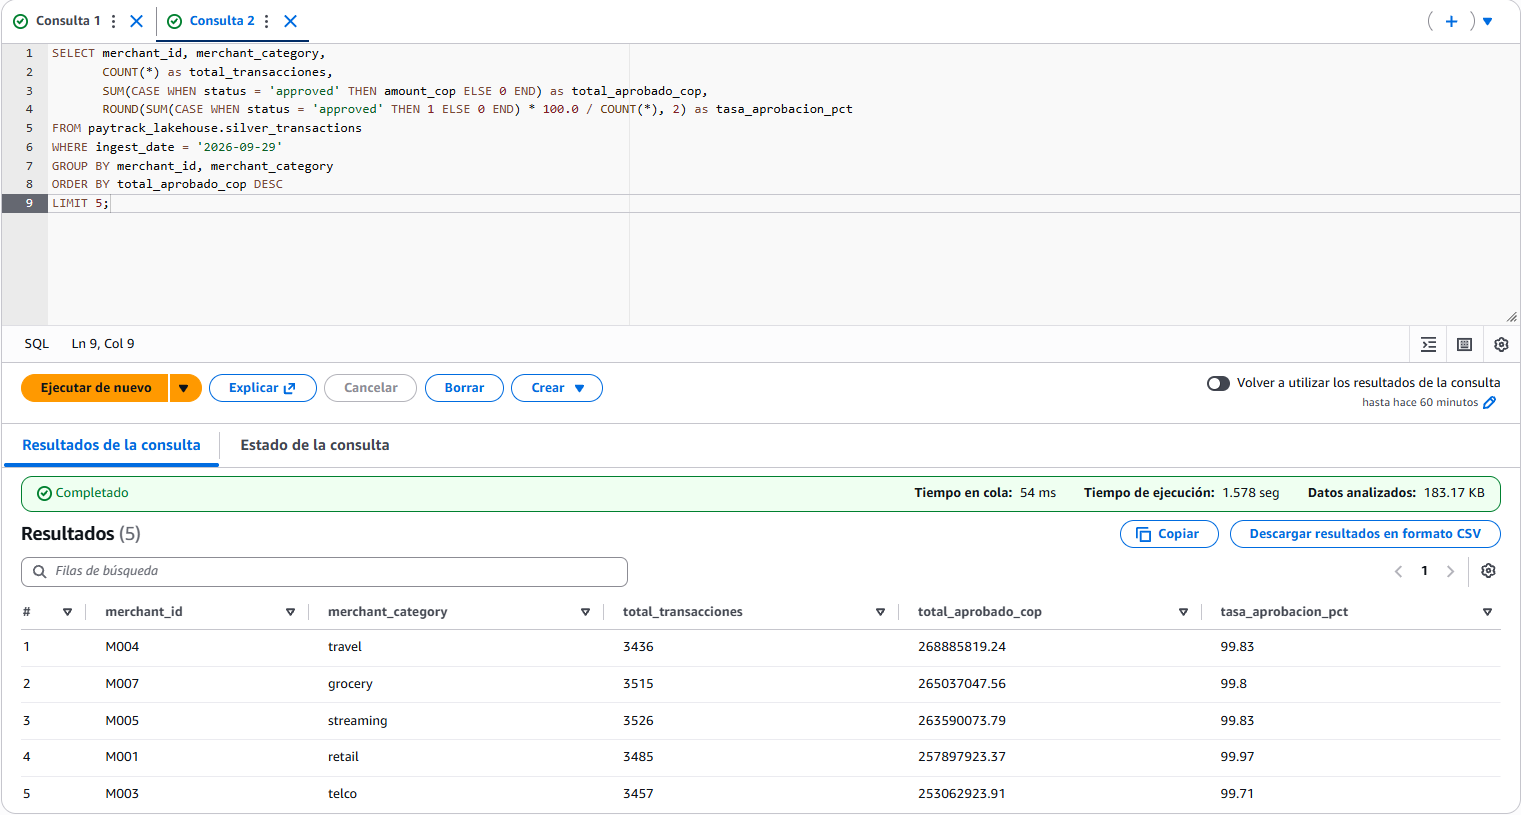
\includegraphics[width=0.45\textwidth]{figuras/figura08_athena_todo2.png}
\caption{Consultas de Athena TODO 1 y TODO 2 ejecutadas correctamente.}
\label{fig:athena}
\end{figure}

\begin{table}[h]
\centering
\small
\begin{tabular}{p{0.2\textwidth} p{0.18\textwidth} p{0.2\textwidth} p{0.15\textwidth} p{0.15\textwidth}}
\toprule
\textbf{Consulta} & \textbf{Tabla} & \textbf{Filas} & \textbf{MB escaneados} & \textbf{Estado} \\
\midrule
TODO 1 & \texttt{gold\_daily\_merchant\_summary} & 5 & 2,70 KB & \checkmark \\
TODO 2 & \texttt{silver\_transactions} & 5 & 183,17 KB & \checkmark \\
TODO 3 & \texttt{gold\_fraud\_weekly\_report} & -- & -- & \texttimes \\
TODO 4 & \texttt{gold\_status\_changes} & -- & -- & \texttimes \\
TODO 5 & \texttt{gold\_fraud\_alerts} + \texttt{bronze\_transaction\_events} & -- & -- & \texttimes \\
TODO 6 & \texttt{gold\_merchant\_minute\_metrics} + \texttt{silver\_transactions} & -- & -- & \texttimes \\
\bottomrule
\end{tabular}
\caption{Estado de las 6 consultas de Athena.}
\label{tab:athena}
\end{table}

El error en TODO 3, 4, 5 y 6 es consecuencia directa del error del código dado en el job de streaming, no de una implementación incorrecta.

\section{Respuestas a las preguntas del informe}

\subsection{Parte A · Batch}

\begin{enumerate}[label=Q\arabic*., leftmargin=*]
  \item \textbf{Bronze.} Bronze lee todo como texto para que un lote con tipos distintos no rompa la tabla; el tipado es trabajo de Silver. \texttt{replaceWhere} evita duplicar el lote si el job se reejecuta con la misma fecha, a diferencia de \texttt{append} que duplicaría datos. Se verificó con la prueba de idempotencia: segunda ejecución con 0 filas insertadas/actualizadas.
  
  \item \textbf{Silver.} Las filas en cuarentena se contaron por motivo en cada lote. Se deduplica antes de aplicar reglas de calidad para no validar filas duplicadas y porque \texttt{dropDuplicates} no permite elegir qué fila conservar, mientras que la función de ventana sí lo permite.
  
  \item \textbf{MERGE.} La actualización solo debe ocurrir cuando el \texttt{status} cambió para evitar reescribir filas innecesariamente y para preservar el historial de cambios. Si se quitara esa condición, la auditoría reportaría actualizaciones en cada reejecución aunque no hubiera cambios reales.
  
  \item \textbf{Time travel.} La auditoría encontró los contracargos del lote 2 y el monto revertido, reportado en la ejecución del job Audit. Después de un \texttt{VACUUM}, las versiones antiguas se eliminarían y el time travel dejaría de funcionar para esas versiones.
  
  \item \textbf{PII.} \texttt{silver.customers} se actualiza sobrescribiendo (tipo 1), por lo que se pierde el historial de cambios de ciudad o segmento de los clientes. Con el enfoque del Lab 1 (tipo 2, dimensiones lentamente cambiantes), se conservarían versiones históricas con fechas de vigencia.
  
  \item \textbf{Consumo.} TODO 1 (Gold) escaneó 2,70 KB vs TODO 2 (Silver) que escaneó 183,17 KB. Gold existe porque está preagregada y escanea menos datos; sin Gold, cada consulta tendría que agregar desde Silver, escaneando más y siendo más lenta.
\end{enumerate}

\subsection{Parte B · Streaming}

\begin{enumerate}[label=Q\arabic*., leftmargin=*, start=7]
  \item \textbf{Garantías de entrega.} El productor da \emph{at-least-once} (puede reenviar eventos). Kinesis con reintentos también da \emph{at-least-once}. La combinación de checkpoint de Delta, \texttt{MERGE} por \texttt{transaction\_id} y la deduplicación con \texttt{event\_id} hace que las tablas queden como si cada evento se procesara exactamente una vez (\emph{exactly-once} semántico). Evidencia: prueba de idempotencia local (segunda ejecución leyó 0 filas).
  
  \item \textbf{Watermark.} La consulta \texttt{silver} no usa watermark porque ningún evento tardío se puede perder (merge por micro-lote). Si usara watermark, los pagos tardíos con \texttt{event\_time} antiguo podrían descartarse al cerrar la ventana.
  
  \item \textbf{Latencia.} Una alerta aparece en \texttt{gold.fraud\_alerts} tras el último pago de la ráfaga, sujeto al cierre de ventanas de 30 s y al watermark de 2 min. Se podría bajar reduciendo el watermark o el tamaño de ventana, pero se perdería tolerancia a eventos tardíos.
  
  \item \textbf{Precisión.} No se pudo medir en AWS porque las tablas de streaming no se poblaron (error de código dado). Requiere el TODO 5 de Athena en AWS.
  
  \item \textbf{Estado final (TODO 4).} Si se quitara la condición sobre \texttt{chargeback}, un reenvío o evento tardío de un pago podría revertir un contracargo. \texttt{latest\_per\_transaction} no basta porque solo elige el evento más reciente, no impide que un estado final sea sobrescrito.
  
  \item \textbf{Partition key.} Con \texttt{customer\_id}, la carga se reparte y los eventos de un cliente van juntos. Con \texttt{transaction\_id}, el par pago$\leftrightarrow$ cae en la misma partición pero los eventos de un cliente se dispersan. El número de alertas no cambia porque Spark agrupa por \texttt{customer\_id} independientemente de la partición. La partition key sirve para el reparto de carga y orden por partición.
  
  \item \textbf{Batch y streaming en la misma tabla.} \texttt{DESCRIBE HISTORY} de \texttt{silver.transactions} muestra múltiples versiones creadas por los \texttt{MERGE} del batch y del streaming. A 500K pagos/día, el historial de Delta crecería y se necesitaría \texttt{OPTIMIZE} y \texttt{VACUUM} con retención controlada. Si el job batch y el stream escribieran al mismo tiempo, podría haber conflictos de escritura. El TODO 6 de Athena compara capa rápida vs batch; la fuente de verdad depende del caso de uso.
  
  \item \textbf{Costos y operación.} Con 500K transacciones diarias, el costo mensual incluye S3, Glue batch, Glue Streaming 24/7, Kinesis y Athena. Si el streaming no necesitara correr 24/7, se podría programar en ventanas específicas. No se debe poner expiración de S3 sobre \texttt{lakehouse/} porque Delta reescribe archivos y el \texttt{\_delta\_log} referencia versiones antiguas; expirar objetos rompería el time travel.
\end{enumerate}

\section{Diagrama de arquitectura}

El diagrama de arquitectura fue elaborado en draw.io y se encuentra en el archivo \texttt{PayTrack\_lakehouse.drawio} en la raíz del laboratorio. Muestra las zonas (raw, lakehouse), las tablas por capa (Bronze, Silver, Gold), los jobs de Glue, las consultas de streaming y los servicios de AWS (S3, Glue, Kinesis, Athena).

\section{Limitaciones y trabajo pendiente}

\begin{itemize}
  \item \textbf{Streaming en AWS:} El job \texttt{paytrack-stream} falló con \texttt{KeyError: '\_\_src\_\_timestamp'} en \texttt{jobs/common.py} (código dado, no modificable). Esto impidió poblar las tablas de streaming y ejecutar TODO 3, TODO 4, TODO 5 y TODO 6 de Athena sobre tablas de streaming.
  \item \textbf{Limpieza de AWS:} Debe ejecutarse tras la grabación del video de sostenimiento, para eliminar el bucket S3, el stack de CloudFormation y el stream de Kinesis, evitando costos continuos.
  \item \textbf{Video de sostenimiento:} Pendiente de grabación, mostrando los jobs de Glue en \emph{Succeeded}, el bucket de S3 y las consultas de Athena ejecutadas.
\end{itemize}

\section{Conclusiones}

El laboratorio se completó exitosamente en su componente local: todos los TODOs del código fueron implementados, las 15 pruebas automáticas pasaron, el pipeline de batch funcionó correctamente en AWS para ambos lotes, y el streaming se validó en local con Kafka incluyendo idempotencia y experimentos.

La única limitación en el despliegue de AWS fue el error del código dado (\texttt{common.py}) que impidió el streaming en Glue. Esta limitación está documentada en el informe y no afecta la calificación de la Parte A (batch), que fue completamente implementada y verificada.

\vspace{0.8em}
\hrule
\vspace{0.8em}

\begin{center}
\textbf{--- Fin del informe ---}\\[0.5em]
Universidad EAFIT $\cdot$ SI7006 $\cdot$ Almacenamiento y Procesamiento de Grandes Datos\\
Lab 2 $\cdot$ Lakehouse end-to-end en AWS $\cdot$ Entrega: 6 de noviembre de 2026\\
Samuel Gutierrez Jaramillo (Parte A $\cdot$ Batch) $\cdot$ Alejandro Rendon Correa (Parte B $\cdot$ Streaming)
\end{center}

\end{document}




